% Standalone working extract; merge into the main paper after editorial review.
\documentclass[conference]{IEEEtran}
\usepackage{cite}
\usepackage{amsmath,amssymb,amsfonts}
\usepackage{algorithmic}
\usepackage{graphicx}
\usepackage{textcomp}
\usepackage{xcolor}
\def\BibTeX{{\rm B\kern-.05em{\sc i\kern-.025em b}\kern-.08em
    T\kern-.1667em\lower.7ex\hbox{E}\kern-.125emX}}
\title{Intent-Aware Sequential Resource Discovery:\\Algorithm and Evaluation Working Extract}
\author{\IEEEauthorblockN{D\'aniel Ficzere\IEEEauthorrefmark{1}\IEEEauthorrefmark{2},
Attila Frank\'o\IEEEauthorrefmark{1}, Gergely Holl\'osi\IEEEauthorrefmark{1},
P\'al Varga\IEEEauthorrefmark{1}, J\'ozsef B\'ir\'o\IEEEauthorrefmark{1}}
\IEEEauthorblockA{\IEEEauthorrefmark{1}Department of Telecommunications and Artificial Intelligence,\\
Budapest University of Technology and Economics, Budapest, Hungary}
\IEEEauthorblockA{\IEEEauthorrefmark{2}AI \& IIoT Division, AITIA International Inc., Budapest, Hungary}}
\begin{document}
\maketitle
\section{Decision Model and Exact Reference}
We consider a single discovery episode, independent domain feasibility,
exact queries and at most one binary refresh per domain. Let $p_i(s)$
denote the posterior feasibility probability of domain $i$ in state $s$,
with $p_i(s)=0$ following a failed query. A query has cost $q_i>0$ and
terminates on success; a refresh has cost $r_i>0$, sensitivity $\alpha_i$
and specificity $\beta_i$. For an unrefreshed domain the positive signal
probability and Bayesian posteriors are
\begin{align}
g_i&=p_i\alpha_i+(1-p_i)(1-\beta_i),\quad h_i=1-g_i,\\
p_i^+&=p_i\alpha_i/g_i,\qquad p_i^-=p_i(1-\alpha_i)/h_i.
\end{align}
Only observations with positive probability require defined posteriors.
Discovery can stop without success if
\begin{equation}
\rho(s)=1-\prod_{i\in D}(1-p_i(s))\leq\varepsilon,
\end{equation}
including any domains irrevocably skipped by the heuristic.
A free, informationless SKIP action restricts subsequent queries and
refreshes without changing the posterior risk. Delaying every such
commitment until termination can reproduce the remaining actions and
observations of any policy using SKIP. Consequently, explicit SKIP is
redundant for exact optimization from an initial state without committed
skips. We retain it in heuristic plans. In a state with committed skips,
exact optimization respects those commitments and includes their risk.
The resulting exact reference DP uses four statuses per active domain:
unrefreshed, positively refreshed, negatively refreshed, and query failure.
Its time and value-table space are $O(N4^N)$ and $O(4^N)$, respectively.
An exact no-refresh reference uses the corresponding $2^N$ subset DP.

\section{Unified IA-OSR Algorithm Family}
Let $H_0(s)$ denote the minimum expected cost over the PSA1 continuation
family. Each plan allows at most one upfront admissible SKIP, at most
one screening module, and queries of remaining domains. A screening
module refreshes an unrefreshed domain and queries it on a positive
signal, skipping it on an admissible negative signal. Fixed modules
are ordered by increasing expected cost-to-success ratio. The screening
module has cost $r_i+g_iq_i$ and success probability $p_i\alpha_i$.
We require feasibility of all possible skipped domains jointly.
With prefix--suffix cost evaluation, computing $H_0$ takes
$O(N^2\log N)$ time. This is a restricted continuation family, not the
full optimal sequential policy.

\subsection{Exact continuation and rollout}
Let $T$ be the Bellman operator, $V^*(s)$ the optimum respecting
commitments in $s$, and $m(s)$ the number of active domains. Define
\begin{equation}
B_K(s)=\begin{cases}V^*(s),&m(s)\leq K,\\H_0(s),&m(s)>K.\end{cases}
\end{equation}
The feasible continuation family is closed under the tails of its plans:
following a negative screening signal, the admissible direct skip and
remaining queries form another allowed plan; following a positive
signal, the remaining query sequence does so. If the initial direct
skip has already been performed it need not be repeated. A permissible
STOP can only improve a continuation. Thus $TH_0\le H_0$.
Since $m(s)$ cannot increase, exact continuation on $m(s)\le K$ gives
$TB_K\le B_K\le H_0$. Write $H_d^{(K)}=T^dB_K$. Monotonicity of $T$ gives
$V^*\le H_2^{(K)}\le H_1^{(K)}\le B_K$.

With $U_d(s,a)=c(s,a)+\mathbb E[H_{d-1}^{(K)}(s')\mid s,a]$
for $d=1,2$, and $H_0^{(K)}=B_K$, the one-step policy minimizes $U_1$.
The selective policy computes all $U_1$ scores and optionally refines
one best candidate per action type (QUERY, REFRESH, SKIP) to $U_2$.
It minimizes the updated scores, leaving all other candidates at $U_1$.
The exact tail reuses cached tables across refresh outcomes and query
failures with identical skip commitments. An active subset can be
represented in a cached superset by query-failure statuses for the
removed domains.

\textit{Guarantee:} let $M(s)$ be the minimum of the mixed scores.
Because $U_2\le U_1$, $M\le H_1^{(K)}$. Inductively over the finite
acyclic state space, the future policy cost is bounded by
$M(s')\le H_1^{(K)}(s')\le B_K(s')$. This proves
\begin{equation}
 V^*(s)\le V^{\pi_{\rm sel}}(s)\le M(s)\le H_1^{(K)}(s).
\end{equation}
The result bounds the policy cost; it does not assert pointwise
improvement over a different rollout policy or a worst-case
approximation ratio. A full two-step policy likewise has a
one-step-or-better upper bound.

\subsection{Adaptive computation}
We use three previously fixed refinement triggers: (i) two individually
admissible skips whose summed log-survival weights lie within 12\% of the
remaining log-risk budget, with at least two refreshable domains;
(ii) the best REFRESH score is within 3\% of the best overall score;
(iii) a refresh has positive net value in the fixed query-only ordering
problem. The third is a trigger rather than a general optimality test.
Refinement is disabled above 16 active domains. The configurations
PSA1, PSA1-E, PSA1-S, and PSA1-A respectively use one-step rollout without
exact tail, one-step rollout with exact tail, selective refinement with
exact tail, and full adaptive refinement with exact tail. All tail
variants use $K=8$ and a 32 MiB LRU tail-table budget. These are engineering
parameters, not optimized constants. With $K$ fixed, one-step and
selective decisions have an $O(N^3\log N)$ time upper bound and unrestricted
full two-step decisions an $O(N^4\log N)$ bound. These refer to one
computed action, not evaluation of an entire decision tree.

\section{Independent Synthetic Validation}
\subsection{Experimental protocol}
We freeze the implementation and parameters before generating 90 new
instances: ten per combination of $N\in\{8,10,12\}$ and three synthetic
families (independent random parameters, extended skip-boundary stress,
and informative refresh with a strict risk tolerance). All policy
expectations are calculated by exact integration of observation branches;
the exact oracle is used only for evaluation except when an algorithm
explicitly invokes its bounded exact tail. We also compare with the
optimal policy subject to disabling REFRESH and the same risk constraint.
The three tail methods are exact at $N=8$; hence we emphasize the 60
larger instances. Paired confidence intervals are obtained by 10,000
bootstrap resamples within the six size--family strata. These intervals
characterize the synthetic design, not a real network population.

\begin{table}[t]
\caption{Mean optimality gap (\%) on fresh models. Ten
instances per family and size; 30 per size.}
\label{tab:gaps}
\centering
\begin{tabular}{rrrrr}\hline
$N$ & PSA1 & E & S & A \\\hline
8 & 5.71 & 0.00 & 0.00 & 0.00\\
10 & 4.97 & 2.84 & 2.35 & 2.11\\
12 & 6.32 & 5.98 & 3.98 & 3.74\\
10--12 & 5.64 & 4.41 & 3.17 & 2.92\\\hline
\end{tabular}
\end{table}
\begin{table}[t]
\caption{Paired mean gap reduction, percentage points ($N=10$--12).}
\centering
\begin{tabular}{lrr}\hline
Transition & Reduction & 95\% CI\\\hline
PSA1 to E & 1.23 & [0.77, 1.75]\\
E to S & 1.24 & [0.54, 2.03]\\
E to A & 1.49 & [0.80, 2.23]\\
S to A & 0.24 & [$-0.17$, 0.66]\\\hline
\end{tabular}
\end{table}
\begin{figure}[t]
\centering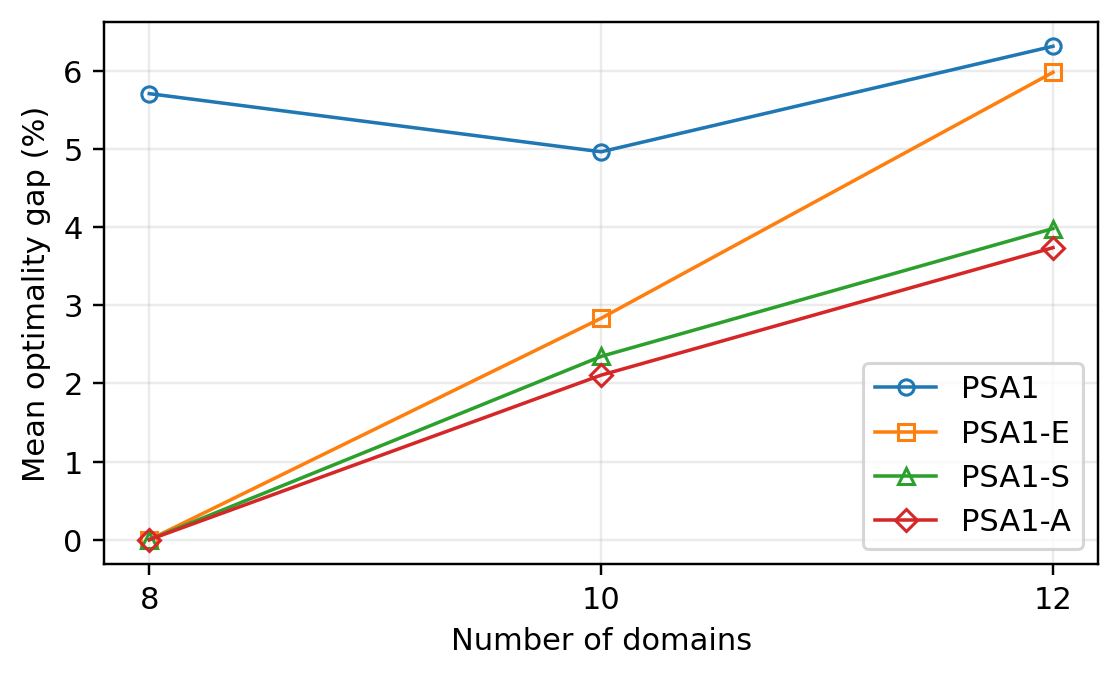
\includegraphics[width=\columnwidth]{fig_gap.png}
\caption{Mean gap by domain count; the hybrids are exact at $N=8$.}
\label{fig:gap}
\end{figure}
\subsection{Quality and value of information}
Tables~\ref{tab:gaps} and the paired comparison show complementary
benefits of exact continuation and selective refinement. The additional
benefit of full adaptive refinement is not resolved by the confidence
interval, which also does not establish equivalence. Relative to the
exact no-refresh reference, PSA1-S saves 18.02\% on average (mean of
per-instance relative savings, $N=10$--12). Its maximum gap is 17.39\%;
the skip-boundary family remains challenging (6.56\% mean gap).
The favorable mean values therefore do not imply a worst-case guarantee.

\begin{table}[t]
\caption{Online action computation time (ms), 120 simulated trajectories
per algorithm at $N=10$--12. Terminal STOP checks excluded from active
per-decision statistics.}
\centering
\begin{tabular}{lrrr}\hline
Method & First median & Active median & Active P95\\\hline
PSA1 & 1.16 & 0.68 & 3.30\\
E & 1.25 & 0.66 & 18.35\\
S & 17.13 & 2.35 & 41.62\\
A & 84.16 & 9.64 & 140.09\\\hline
\end{tabular}
\end{table}
\begin{figure}[t]
\centering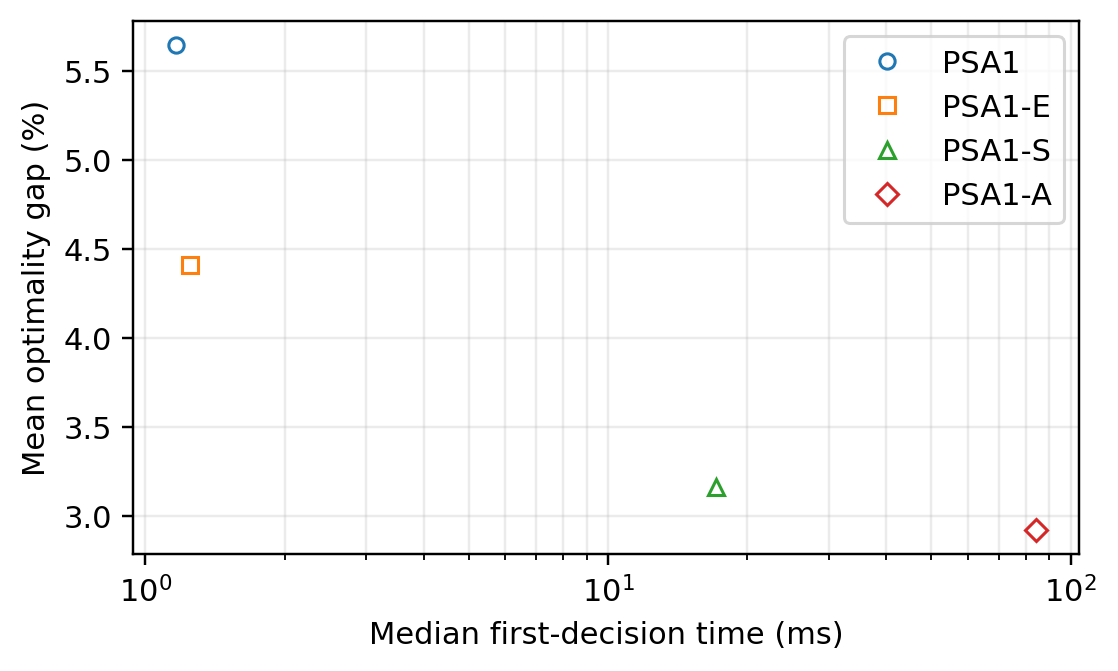
\includegraphics[width=\columnwidth]{fig_tradeoff.png}
\caption{Mean gap and median first-decision computation time at $N=10$--12.}
\end{figure}
\subsection{Online computation and scaling}
We sample two independent feasibility-and-observation realizations per
model, reuse each realization across algorithms, and time decisions
along the realized trajectory rather than the full policy tree. Each
trajectory starts with an empty cache; warm JIT compilation is excluded.
The 720 trajectories satisfy the model-based posterior STOP constraint
within numerical tolerance, but there are too few unsuccessful
terminations to estimate an empirical conditional miss rate reliably.
The median first action of PSA1-S is nearly five times faster than
PSA1-A in the $N=10$--12 sample.
\begin{figure}[t]
\centering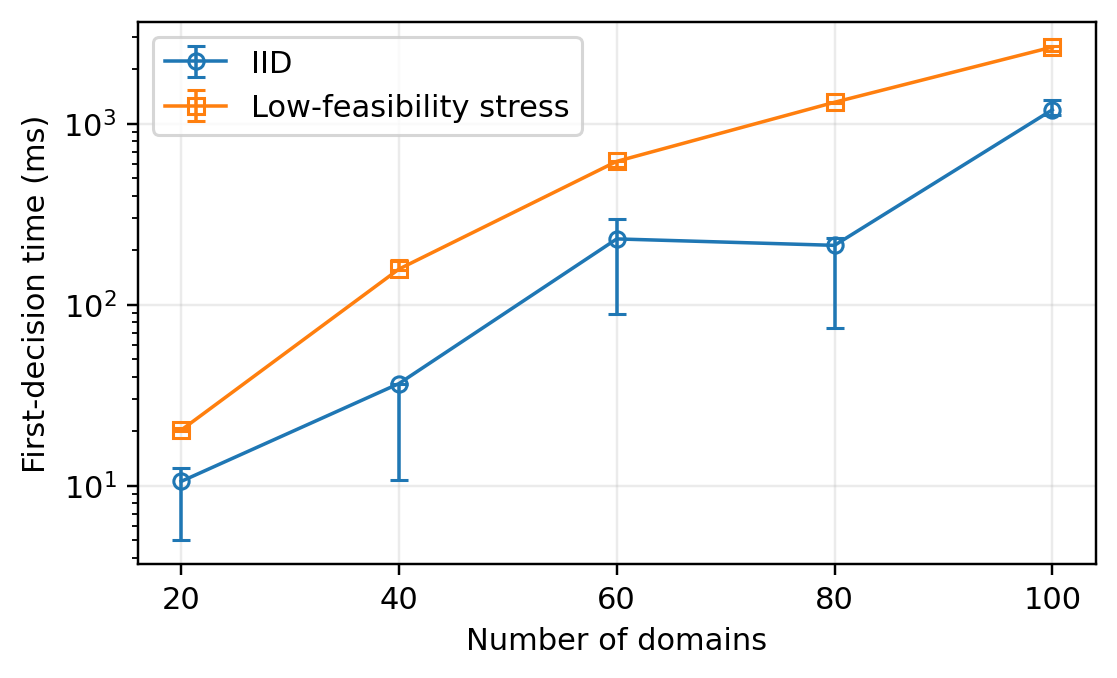
\includegraphics[width=\columnwidth]{fig_scaling.png}
\caption{Initial decision time for 20--100 domains. Median and observed
range over three instances per family and size. All configurations use
the one-step computation at these initial sizes.}
\end{figure}
Large-scale computation is evaluated at $N\in\{20,40,60,80,100\}$
with three random and three low-feasibility stress instances per size.
The latter use $p_i\sim U[0.018,0.026]$, $q_i\sim U[4,12]$,
$r_i/q_i=0.2$, $\alpha_i=\beta_i=0.95$, and $\varepsilon=0.1$.
At 100 domains the median first decision requires 1.19 s for the random
family and 2.64 s for the stress family on the test host. This is a
root-only measurement, not large-scale policy-quality or full episode
validation. Times depend on hardware and implementation and exclude
network communication. Large stress cases remain unsuitable for strict
real-time deadlines with the current implementation.
\section{Interpretation}
The selective configuration is a natural default for the studied
accuracy--computation tradeoff, with one-step exact-tail rollout as a
lower-computation alternative. The algorithms assume calibrated
beliefs and independent static domain feasibility. The synthetic
results do not establish performance on correlated or drifting
workloads, nor do they replace the existing calibration stress tests
and complementary trace-driven pilot.
\end{document}
